\documentclass[10pt]{article}

\usepackage[margin=0.9in]{geometry}
\usepackage{amsmath}
\usepackage{booktabs}
\usepackage{graphicx}
\usepackage[colorlinks=true,linkcolor=black,citecolor=black,urlcolor=black]{hyperref}

\setlength{\parskip}{0.5em}
\setlength{\parindent}{0pt}

\title{When does an intrusion detector catch an attack it has never seen?\\
A detection map on NSL-KDD and CIC-IDS2017}
\author{Luca Accomando\\Catawba College}
\date{}

\begin{document}
\maketitle

\begin{abstract}
I ask when a network intrusion detector catches an attack type that was absent from its training data, and
whether the type's position relative to normal and known attack traffic tells us in advance. I compare a
Random Forest with three anomaly detectors (Isolation Forest, LOF, One-Class SVM) on NSL-KDD and CIC-IDS2017.
Alert thresholds are set on a validation split at fixed false-alarm targets, so detectors are compared at
operating points and not at a best-F1 threshold. For every attack type I measure its distance from normal
traffic ($x$) and from the other attack types ($y$). Across 30 NSL-KDD types, $x$ is rank-correlated with
recall for both the forest (Spearman 0.74) and normal-only Isolation Forest (0.62); $y$ is not
correlated in the direction I expected, and neither position predicts the recall of a single type
better than the mean of the other types. On NSL-KDD the forest's false-alarm rate on the test file is 12.6\% for a
5\% target; on CIC-IDS2017 it holds its target (4.5\%). The anomaly detectors depend strongly on the feature
transform. An earlier result of mine, that Isolation Forest beat Random Forest, came from a threshold tuned on
test labels, and I report that correction in the paper.
\end{abstract}

\section{Introduction}

Most evaluations of machine-learning intrusion detectors draw training and test flows from the same
distribution. A deployed detector meets attack types and traffic it was not trained on
\cite{sommer2010,arp2022}. Anomaly detectors are often proposed for this case, since they need no attack
labels. Supervised detectors are expected to fail on new attacks. I wanted to check how much of that is true
at an operating point a defender could actually use, and whether the answer can be predicted from the data.

The question is: \emph{when does a network intrusion detector catch an attack type it has never seen, and can we
tell in advance which new attacks it will miss?} I state three hypotheses and test them rather than assume
them.
\begin{enumerate}
\item A supervised detector catches a new attack type when it resembles the types it was trained on.
\item An anomaly detector catches a new attack type when it lies far from normal traffic.
\item Types that lie close to normal traffic and far from every known attack type are missed by both, at a
reasonable false-alarm rate (the blind spot).
\end{enumerate}

The main tool is a detection map. Each attack type is a point $(x, y)$ computed from the training data only,
where $x$ is its distance from normal flows and $y$ its distance from the nearest other attack types. I plot
recall against position and test whether position predicts recall. The study also repeats several evaluation
mistakes listed by Arp et al.\ \cite{arp2022} and measures how far each moves the headline number.

\section{Method}

\subsection{Data and protocol}

NSL-KDD \cite{tavallaee2009} has 125,973 training flows (47\% attacks) and 22,544 test flows (57\% attacks). The
test file holds 17 attack types that never occur in the training file (3,750 flows, 29\% of the test
attacks). I use the 38 numeric columns; the three categorical columns are dropped in the main results. NSL-KDD
derives from 1998 DARPA traffic, so it is dated and its attacks are simulated.

CIC-IDS2017, in the corrected release of Engelen et al.\ \cite{engelen2021}, gives a cleaner novelty test.
Monday to Wednesday contain FTP-Patator, SSH-Patator and five DoS types. Thursday and Friday contain only
attack types that never occur earlier: port scans, DDoS, botnet, web attacks and infiltration. Training and
validation come from Monday to Wednesday, split in 10-minute blocks so that one burst does not land on both
sides; the test set is Thursday and Friday. Flows labelled ``attempted'' are relabelled normal, as the authors
recommend. I use 82 features, drop ports, and cap the number of flows per class per seed.

For each of five seeds, a stratified 20\% validation split is drawn from the training file. Models and the
scaler are fit on the other 80\%. The validation split sets each detector's alert threshold, which is then
applied unchanged to the test set. Isolation Forest, LOF and One-Class SVM \cite{liu2008,breunig2000,
scholkopf2001} train without labels, and Random Forest \cite{breiman2001} uses labels. The unsupervised
detectors are run in two ways: trained on all training flows, and on normal flows only. The normal-only variant
selects the normal rows with labels, so it needs a clean normal capture in practice. The validation split uses
labels, only to choose thresholds.

\subsection{Operating points}

A detector's best-F1 threshold depends on the attack share of the validation set, so I do not compare
detectors there. The main operating points are thresholds at 1\% and 5\% false alarms on the validation normal
flows. I report recall at that threshold and the false-alarm rate the same threshold produces on the test set,
since the two can differ under distribution shift. Precision is also re-weighted to a 1\% attack base rate,
following Axelsson \cite{axelsson1999}, because 57\% attacks flatters every detector's precision.

\subsection{Leave-one-attack-type-out}

On the training file alone, each attack type $T$ with at least 20 flows is removed from training and validation.
Its flows form the attack side of a test set, next to 20\% of the normal flows that no model or threshold
saw. Test normals come from the same file as training, so the test false-alarm rate stays near the target,
which the NSL-KDD test file cannot give. I also hold out whole categories (DoS, Probe, R2L, U2R). Types
related to $T$ can remain in training, so this is not a strict zero-day test.

\subsection{Detection map}

In the feature space of the training split, $x$ for a type is the median, over the type's flows, of the mean
distance to the 5 nearest normal training flows. $y$ is the same quantity to the nearest flows of the other known
attack types, with the type itself excluded. Points come from the held-out types and from the 17 types that
are unseen in the NSL-KDD test file. Grouping test rows by type is for analysis only. I test whether position
predicts recall with Spearman correlations (bootstrap intervals over types) and with leave-one-type-out
prediction of recall from $(x, y)$ against a constant baseline.

\section{Results on NSL-KDD}

\subsection{Operating points on the test file}

Table~\ref{tab:fixed} gives recall at the validation targets. The forest recalls the most at every target, but
its threshold does not transfer to the test file: a 1\% target gives a 6.4\% false-alarm rate there, and a 5\%
target gives 12.6\%. Normal-only Isolation Forest stays near its target (0.7\% and 2.2\%) and recalls 62\% of
unseen attack flows at the 5\% target, against 91\% for the forest at 12.6\% false alarms. Because the
false-alarm rates differ, I cannot say that either wins at equal false-alarm rate on this test file. That
comparison would need thresholds that do not use test labels, and NSL-KDD has no benign-only validation set
for them. Label-free quantile thresholds on validation scores did not help, because validation is 47\% attacks
and the quantile lands where the attacks are.

\begin{table}[t]
\centering\small
\begin{tabular}{llrrrrr}
\toprule
Detector & Training & Target & Test FPR & Recall all & Seen & Unseen\\
\midrule
Isolation Forest & normal only & 1\% & 0.007 & 0.540 & 0.595 & 0.407\\
Isolation Forest & normal only & 5\% & 0.022 & 0.638 & 0.644 & 0.622\\
Isolation Forest & all flows & 5\% & 0.014 & 0.258 & 0.137 & 0.552\\
Random Forest & labels & 1\% & 0.064 & 0.818 & 0.852 & 0.737\\
Random Forest & labels & 5\% & 0.126 & 0.960 & 0.979 & 0.913\\
One-Class SVM & normal only & 5\% & 0.079 & 0.661 & 0.783 & 0.366\\
LOF & normal only & 5\% & 0.102 & 0.474 & 0.554 & 0.281\\
\bottomrule
\end{tabular}
\caption{NSL-KDD, recall at a validation false-alarm target, mean of 5 seeds. Test FPR is the false-alarm rate of
the same threshold on KDDTest+.}
\label{tab:fixed}
\end{table}

Two caveats on the headline. First, training Isolation Forest on all flows, attacks included, changes it a lot:
at its best validation F1 its false-alarm rate falls from 36\% to 6.5\% when trained on normal flows only,
and ROC-AUC rises from 0.880 to 0.927. Second, LOF trained on all flows flags 99.7\% of normal test flows at its
best validation F1, so its F1 of 0.726 is the flag-all score at this base rate and not a result.

\subsection{Leave-one-attack-type-out}

Table~\ref{tab:loo} shows the matched comparison. At a 5\% target the test false-alarm rate is between 0.041
and 0.051 for every model, so the recalls are comparable. The forest leads on DoS, Probe and U2R. On R2L its lead over normal-only
LOF (0.473 against 0.467) is not meaningful. Single types show the same split: the forest recalls teardrop,
pod and warezmaster at 1.000 when they are held out, and normal-only Isolation Forest recalls 0.105, 0.045 and
0.050. The forest's weakest held-out type is warezclient (0.475). Normal-only models never see an attack, so
holding one out only moves their threshold, and their recall reflects how far the type lies from normal traffic.

\begin{table}[t]
\centering\small
\begin{tabular}{lrrrr}
\toprule
Held out (types) & Random Forest & IF, normal only & OC-SVM, normal only & LOF, normal only\\
\midrule
DoS (6) & 0.993 & 0.909 & 0.938 & 0.518\\
Probe (4) & 0.966 & 0.542 & 0.761 & 0.733\\
R2L (8) & 0.473 & 0.169 & 0.441 & 0.467\\
U2R (4) & 0.931 & 0.235 & 0.669 & 0.550\\
\bottomrule
\end{tabular}
\caption{Leave-one-attack-type-out on KDDTrain+: recall at a 5\% validation false-alarm target, 5 seeds.}
\label{tab:loo}
\end{table}

\subsection{The detection map}

Figure~\ref{fig:map} shows the 30 types (13 held out, 17 unseen in the test file). Twenty-seven lie at $x$ below
12. Three KDDTest+ types (xterm, sqlattack, xsnoop) lie far out, at $x$ between 64 and 145. In the test file, 30 unseen
attack flows are exact copies of a normal training flow: 28 snmpgetattack, one named and one snmpguess. The
blind spot is therefore not only about exact copies; it is about types that sit very close to normal traffic.

\begin{figure}[t]
\centering
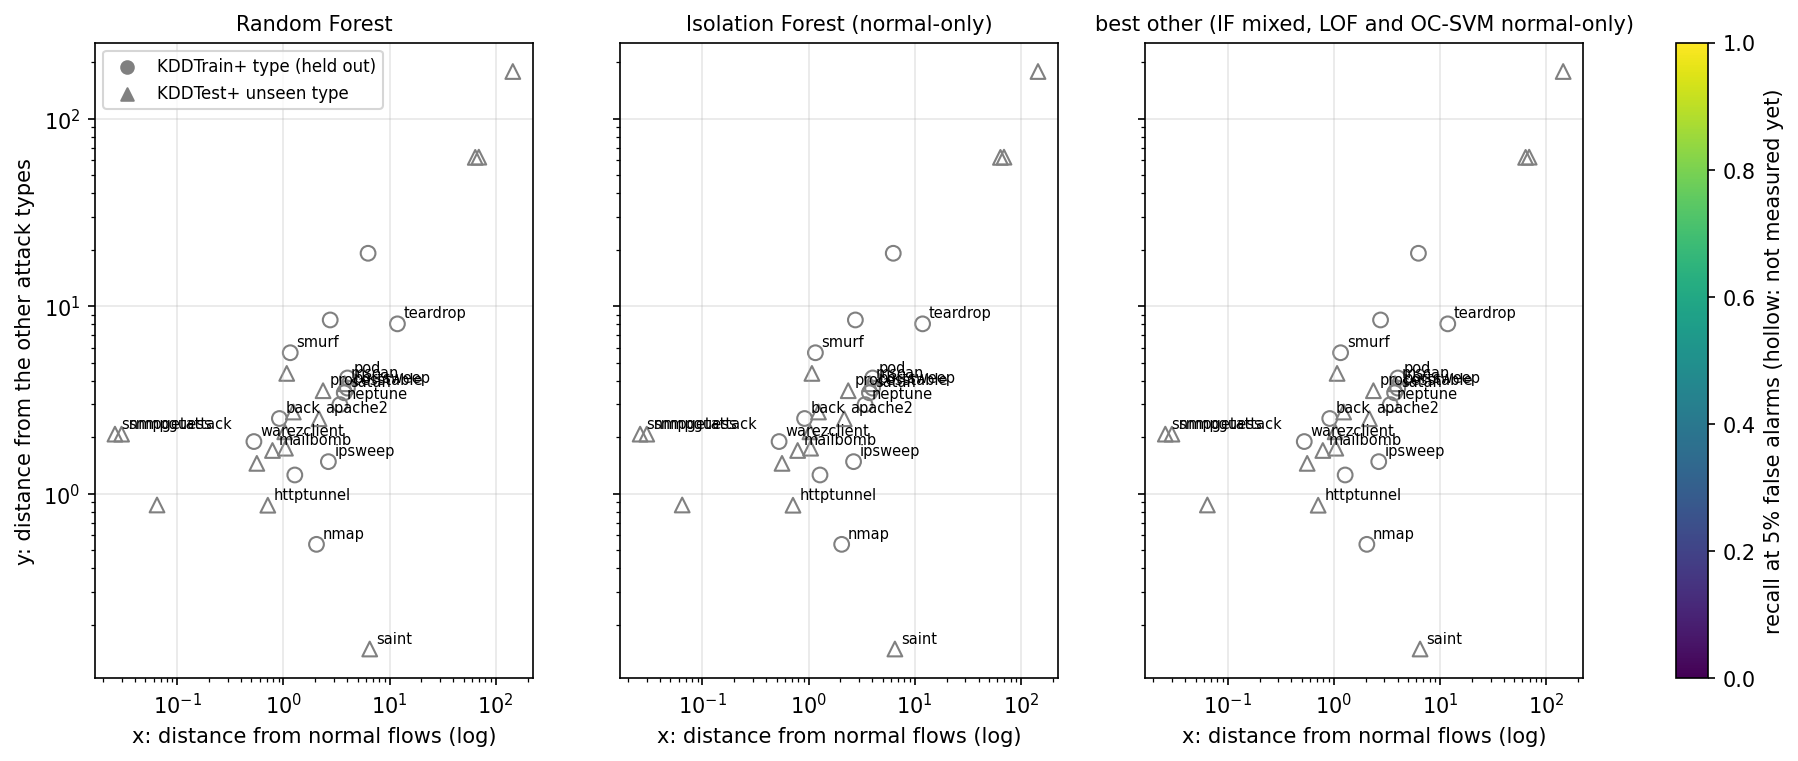
\includegraphics[width=\textwidth]{../results/detection_map.png}
\caption{NSL-KDD detection map. Each point is an attack type, coloured by recall at the 5\% validation target.
Circles are held-out KDDTrain+ types, triangles are types that appear only in KDDTest+. Axes are logarithmic.}
\label{fig:map}
\end{figure}

Table~\ref{tab:map} gives the rank correlations. Distance from normal traffic goes with recall for both the
forest and normal-only Isolation Forest. The held-out group alone is too small to support a conclusion (13
types, intervals reach below zero). The pooled groups mix two operating points, because held-out recall is at a
matched 5\% false-alarm rate and unseen recall is at a drifted one, so I also give them separately.

\begin{table}[t]
\centering\small
\begin{tabular}{lrrr}
\toprule
Group (types) & $x$ vs forest & $x$ vs IF, normal only & $y$ vs forest\\
\midrule
All (30) & 0.74 [0.48, 0.89] & 0.62 [0.33, 0.84] & 0.41 [0.04, 0.70]\\
Held out (13) & 0.48 [$-$0.18, 0.87] & 0.37 [$-$0.25, 0.96] & 0.37 [$-$0.26, 0.83]\\
Unseen in KDDTest+ (17) & 0.76 [0.35, 0.94] & 0.68 [0.22, 0.91] & 0.31 [$-$0.20, 0.75]\\
\bottomrule
\end{tabular}
\caption{Spearman correlation between map position and recall at the 5\% target, with 95\% bootstrap
intervals over types.}
\label{tab:map}
\end{table}

For the three hypotheses: the second is supported in direction. The first is not supported in sign, because
types far from the known attacks are not caught less by the forest; the pooled correlation of $y$ with forest recall is
positive (0.41), with an interval that barely excludes zero. The third, the blind spot, is not tested by
these correlations. Position also does not predict the recall of an individual type out of sample: leave-one-type-out
mean absolute error over 30 types is 0.17 for the forest against 0.17 for the mean of the other types, and
0.33 against 0.30 for normal-only Isolation Forest. The map explains the order of the types, not their recall.
The $x$ order is stable across neighbour counts (Spearman 0.97 at $k=1$, 0.99 at $k=20$) but moves when the
categorical columns are one-hot encoded (0.88 to 0.92), so the map depends partly on that choice.

\subsection{Forest plus an anomaly detector}

I also evaluated, as a comparison and not as a new method, a forest whose alerts are extended by an anomaly detector's alerts
on the flows the forest calls normal, sharing one 5\% validation false-alarm budget. On the test file
the forest alone has 0.126 false alarms and 0.913 recall on unseen types. Forest plus normal-only Isolation
Forest has 0.107 and 0.866. Splitting the budget shrinks the forest's share, and the recall it loses is larger
than what the detector adds. I measured no gain.

\section{A second dataset: CIC-IDS2017}

Table~\ref{tab:cic} gives recall at the 5\% target over all Thursday and Friday attacks. The forest ranks flows
best (ROC-AUC 0.990) and holds its target (test false-alarm rate 0.045), unlike on NSL-KDD. It catches every new type except botnet (0.54).
The anomaly detectors depend heavily on the feature space. I show the raw features and
$\mathrm{sign}(x)\log(1+|x|)$ (slog1p). The validation rule, mean validation PR-AUC of the three detectors, picks raw
features for detectors trained on all flows and slog1p for normal-only training, while the test days favour
slog1p for all three. I report both and do not choose by test. Raw Isolation Forest recalls 4\% of the new
attacks and 65\% with slog1p. I did not test why the transform matters so much; heavy-tailed columns are the
obvious suspect.

\begin{table}[t]
\centering\small
\begin{tabular}{llrrr}
\toprule
Detector & Features & ROC-AUC & Test FPR & Recall\\
\midrule
Random Forest & either & 0.990 & 0.045 & 0.987\\
IF, normal only & raw & 0.843 & 0.044 & 0.043\\
IF, normal only & slog1p & 0.951 & 0.050 & 0.648\\
LOF, normal only & raw & 0.944 & 0.056 & 0.433\\
LOF, normal only & slog1p & 0.988 & 0.062 & 0.974\\
OC-SVM, normal only & raw & 0.928 & 0.045 & 0.431\\
OC-SVM, normal only & slog1p & 0.955 & 0.049 & 0.974\\
\bottomrule
\end{tabular}
\caption{CIC-IDS2017, recall at the 5\% target over all test attacks, 5 seeds. Recall is dominated by the three
types with 10,000 flows each.}
\label{tab:cic}
\end{table}

Botnet (736 flows) is missed by every unsupervised detector in both spaces (recall 0.06 to 0.07), and SQL
injection (13 flows) is missed by Isolation Forest and One-Class SVM in both. These are the two types closest to
normal traffic on the map (raw $x = 0.65$ and $0.97$), which fits the blind-spot hypothesis, but two types,
one with 13 flows, are too few to support it. On the map of 14 types, $x$ is correlated with recall for normal-only
Isolation Forest (Spearman 0.89 [0.60, 0.99] on raw features, 0.60 [0.07, 0.91] with slog1p) and with the forest
(0.72 raw, 0.46 with slog1p, the latter interval including zero). $y$ does not predict forest recall (0.36 raw, 0.06
slog1p, intervals including zero). Leave-one-type-out error for normal-only Isolation Forest is 0.17 against 0.40
for the mean of the other types on raw features, so position does predict the anomaly detector out of sample here, unlike on NSL-KDD. The four DoS types sit close together on the map, so leaving one out leaves near copies of
it, which flatters that test. The ranking of the 14 types differs between the two feature spaces
(Spearman 0.51), so the map is not a property of the attacks alone.

Leave-one-type-out on Monday to Wednesday shows the same dependence for the forest. It recalls 0.92 to 1.00 of each single DoS type
and FTP-Patator, where a relative remains in training. It falls to 0.60 for SSH-Patator, 0.27 when both Patator
types are out, and 0.15 when all DoS types are out. This fits the first hypothesis for whole families, although
the map's $y$ axis did not predict it. The anomaly detectors do not follow that pattern.

\section{How much the evaluation choices move the numbers}

Table~\ref{tab:pitfalls} repeats some of the mistakes listed by Arp et al.\ \cite{arp2022}. Each row changes one
choice and reports the headline with and without it.

\begin{table}[t]
\centering\small
\begin{tabular}{llrrr}
\toprule
Choice & Model & With & Without & Shift\\
\midrule
threshold chosen on test labels (F1) & Random Forest & 0.936 & 0.796 & $+$0.139\\
threshold chosen on test labels (F1) & Isolation Forest & 0.838 & 0.835 & $+$0.003\\
precision at test base rate, vs 1\% & Random Forest & 0.970 & 0.196 & $+$0.773\\
default threshold, vs validation threshold (F1) & Isolation Forest & 0.458 & 0.835 & $-$0.377\\
fixed 5\% target, test FPR vs target & Random Forest & 0.126 & 0.050 & $+$0.076\\
unseen recall at 5\%, NSL-KDD vs CIC-IDS2017 & Isolation Forest & 0.552 & 0.011 & $+$0.541\\
unseen recall at 5\%, NSL-KDD vs CIC-IDS2017 & Random Forest & 0.913 & 0.987 & $-$0.074\\
\bottomrule
\end{tabular}
\caption{Effect of single evaluation choices. The last two rows use all training flows and raw features.}
\label{tab:pitfalls}
\end{table}

The first row corrects my own earlier claim. A version of this project reported Isolation Forest beating Random
Forest, and that comparison tuned only one model's threshold on test labels. With the same treatment for both, the forest wins (0.936
against 0.838). Without it, the forest's F1 falls to 0.796, and the forest's F1 at a 2.8\% false-alarm rate is
not comparable with Isolation Forest's at 6.5\%. Moving to a second dataset moves the conclusion about Isolation
Forest trained on all flows from catching about half of the unseen types to almost none.

\section{Limitations}

\begin{itemize}
\item NSL-KDD is dated and simulated. CIC-IDS2017 is one lab capture from 2017, and its test days differ from the
training days by new attack types and by the day itself; I cannot separate the two. Its web attack and
infiltration types have 13 to 104 test flows.
\item Thresholds use labels from a validation split. A label-free threshold that targets a false-alarm rate needs a
benign-only validation set, which I did not have, so a matched comparison on the NSL-KDD test file is missing.
\item The map has 13 to 30 types, and its intervals are wide. Held-out types still have relatives in training.
\item The anomaly detectors' results depend on the feature transform, and validation and test disagree about it.
\item The capture and feature-extraction pipeline in the repository uses a different 9-feature set, so these
results say nothing about it. It has been checked on a synthetic capture only.
\end{itemize}

\section{Conclusion}

Distance from normal traffic goes with which unseen attack types an anomaly detector catches, on two datasets.
Position on the map does not predict the recall of an individual type, and the forest's recall falls when a whole family of related types is held out (CIC-IDS2017). The false-alarm rate that a threshold gives on shifted data can be 2.5 times its target, so the
fixed-target comparisons here hold within a protocol and not across files. Code, numbers and the scripts that
produce them are in the repository.

\begin{thebibliography}{99}\small

\bibitem{arp2022} D.~Arp, E.~Quiring, F.~Pendlebury, A.~Warnecke, F.~Pierazzi, C.~Wressnegger, L.~Cavallaro,
K.~Rieck. Dos and Don'ts of Machine Learning in Computer Security. USENIX Security Symposium, 2022.

\bibitem{axelsson1999} S.~Axelsson. The base-rate fallacy and its implications for the difficulty of intrusion
detection. ACM Conference on Computer and Communications Security, 1999.

\bibitem{breiman2001} L.~Breiman. Random Forests. Machine Learning 45(1), 2001, pp.~5--32.

\bibitem{breunig2000} M.~M.~Breunig, H.-P.~Kriegel, R.~T.~Ng, J.~Sander. LOF: Identifying Density-Based Local
Outliers. ACM SIGMOD, 2000, pp.~93--104.

\bibitem{engelen2021} G.~Engelen, V.~Rimmer, W.~Joosen. CICIDS2017 relabelling. IEEE Security and Privacy
Workshops, 2021, pp.~7--12. DOI 10.1109/SPW53761.2021.00009.

\bibitem{liu2008} F.~T.~Liu, K.~M.~Ting, Z.-H.~Zhou. Isolation Forest. IEEE International Conference on Data
Mining, 2008, pp.~413--422.

\bibitem{scholkopf2001} B.~Sch\"olkopf, J.~C.~Platt, J.~Shawe-Taylor, A.~J.~Smola, R.~C.~Williamson. Estimating the
Support of a High-Dimensional Distribution. Neural Computation 13(7), 2001, pp.~1443--1471.

\bibitem{sommer2010} R.~Sommer, V.~Paxson. Outside the Closed World: On Using Machine Learning for Network
Intrusion Detection. IEEE Symposium on Security and Privacy, 2010. DOI 10.1109/SP.2010.25.

\bibitem{tavallaee2009} M.~Tavallaee, E.~Bagheri, W.~Lu, A.~A.~Ghorbani. A Detailed Analysis of the KDD CUP 99 Data
Set. IEEE Symposium on Computational Intelligence for Security and Defense Applications, 2009, pp.~1--6.

\end{thebibliography}

\end{document}
